\newpage
\section{Cloud-Computing - Gewitterwolke oder Schattenspender?}
Der Begriff Cloud bzw. Cloud-Computing wurden in den letzten paar Jahren immer populärer. Das Interesse an der mystischen Wolke und deren Konzept ist stetig gewachsen und ein Ende ist nicht in Sicht. Gerade in den letzten Monaten, während den Enthüllungen Edward Snowdens über die Machenschaften der Geheimdienste, bekam die Cloud aber auch einen bitteren Beigeschmack. Für Privatanwender und Unternehmen gleichermassen stellt sich die Frage, ob ihre Geheimnisse bei Anbietern wie Microsoft, Google oder Amazon sicher sind. Um diese Frage überhaupt beantworten zu können, muss man das Konzept von Cloud-Computing verstehen.

\subsection{Was ist Cloud-Computing?}
Cloud-Computing bezeichnet das Modell, IT-spezfifische Dienste einem Kunden abstrahiert über ein Netzwerk zur Verfügung zu stellen und an dessen Bedarf anzupassen. Der Zugriff auf die Dienste soll dabei möglichst bequem und allgegenwärtig möglich sein. Die zur Verfügung gestellten Dienste können dabei von hardwareseitiger Natur sein (Rechenkapazitäten, Netzwerkkapazitäten, Rechenleistung) oder in Form von fertiger Software angeboten werden\footnote{\url{http://csrc.nist.gov/publications/nistpubs/800-145/SP800-145.pdf}} \footnote{\url{https://de.wikipedia.org/wiki/Cloud-Computing}}.
Die zuvor erwähnte Abstraktion ist dabei ein sehr wichtiger Punkt. Privatpersonen oder Unternehmen, die ein funktionierendes System oder eine funktionierende Software wünschen, ohne sich mit den technischen Aspekten auseinandersetzen zu müssen, kommen so voll auf ihre Kosten. Die Preise für die verschiedenen Dienste werden oft in Form von Abonnements angeboten und dabei zusätzlich an den Bedarf angepasst. Der Kunde erhält somit ein auf ihn zugeschnittenes Paket, das er nur noch einsetzen muss.
\\
\\
Das Konzept scheint aufzugehen und der Beweis dafür sind die unzähligen Firmen/Dienste, welche in den letzten Jahren, wie Pilze im Wald, aus dem Boden spriessen:
\begin{itemize}
\item SkyDrive (Online-Speicher, Microsoft)
\item Office 365 (Online nutzbare Office Suite, Microsoft)
\item Google Drive (Online-Speicher, Google) 
\item Google Docs (Online Office Suite mit beschränktem Funktionsumfang, Google)
\item Dropbox (Online-Speicher, Dropbox Inc.)
\item Evernote (Online-Notizverwaltung, Evernote Corporation)
\item ownCloud (Online-Speicher, ownCloud Inc./Community)
\item u.v.m.
\end{itemize}

Die obige Aufzählung ist nur ein kleiner Teil des tatsächlichen Angebots. Die Wolke wächst kontinuierlich an. Aber welche Risiken sind mit Cloud-Diensten verbunden? Welchen Preis - von Geld einmal abgesehen - muss eine Privatperson oder ein Unternehmen bezahlen, um in den Genuss der Cloud zu kommen?

\subsection{Alltagsbeispiel – Microsoft Office 365}
Eines der wohl am meisten verwendeten Programme in der Geschäftswelt und auch privat ist die Office Suite von Microsoft. Diese wird nun, dem Trend folgend, seit ungefähr zwei Jahren ebenfalls über die Cloud angeboten. Die Vorteile dabei scheinen, zumindest auf den ersten Blick, ein Kaufgrund zu sein:

\begin{itemize}
\item Stets neueste Version der Programme
\item Auf bis zu 5 Geräten nutzbar
\item Offline und online nutzbar, Installation nicht zwingend erforderlich
\item 20 GB+ Online-Speicher, um Dokumente zu speichern und zu synchronisieren
\item Monatlich oder jährlich bezahlbar
\item 60+ „Skype-Minuten“ monatlich in alle Länder (Skype ist eine Telefonie-Software, welche über das Internet kommuniziert)\footnote{\url{https://office.microsoft.com/de-ch/products/microsoft-office-365-home-premium-kaufen-FX102853961.aspx}}
\end{itemize}

Das Ziel ist es natürlich, Office hauptsächlich in Verbindung mit der Cloud zu nutzen. Nur dann kann man von überall seine Dokumente verwalten, ohne dass man die Programme auf den jeweiligen Computern installiert haben muss. Die Daten landen dann alle in der Cloud, womit eigentlich die Server von Microsoft gemeint sind. Microsoft bietet dafür einen eigenen Online-Speicher-Dienst namens „Sky-Drive“ an. Ein Käufer von Office 365 erhält also kurz gesagt die volle Funktionalität, ohne sich viel mit technischen Fragen auseinandersetzen zu müssen. Das Angebot richtet sich dabei nicht nur an Privatpersonen, sondern auch an Firmen, wobei natürlich die Ausstattung und die Preise variieren.
\\
\\
Das obige Beispiel ist nur ein Angebot von vielen. Auf den ersten Blick scheint es auch nichts Schlechtes daran zu geben und natürlich schreiben die jeweiligen Anbieter die mit ihren Diensten verbundenen Risiken nicht auf ihre Flaggen. Schaut man aber genauer hin, tauchen Fragen auf, die gerade mit der zurzeit laufenden Debatte um Datenschutz und Anonymität im Netz vieles überschatten, was zuvor rosig wirkte.

\subsection{Gewitterwolke statt Schattenspender?}
Das grosse Wort, das bei Debatten über die Risiken von Cloud Computing im Raum steht und immer öfter auch ausgesprochen wird, lautet Datenschutz. Datenschutz kann je nach Betrachtungsweise verschiedene Dinge ansprechen:

\begin{itemize}
\item Schutz vor missbräuchlicher Datenverarbeitung
\item Schutz des Rechts auf informationelle Selbstbestimmung
\item Schutz des Persönlichkeitsrechts bei der Datenverarbeitung
\item Schutz der Privatsphäre\footnote{\url{https://de.wikipedia.org/wiki/Datenschutz}}
\end{itemize}

Einfach ausgedrückt, ist das Ziel von Datenschutz der Schutz aller persönlicher Daten eines jeden Bürgers. Jeder Bürger soll selbst entscheiden können, welche seiner persönlichen Daten wem zugänglich sind, zu welchem Zeitpunkt dies geschieht und in welcher Art. Die Frage lautet nun, ob Cloud-Dienste diesen Schutz gewährleisten können oder ob er allein in der Natur der Cloud-Dienste schon aufgehoben ist. Da die Anbieter und ihre Rechenzentren sich oftmals in einem anderen Land oder gar auf einem anderen Kontinent befinden als der Kunde, kann dieser kaum kontrollieren, was mit seinen Daten wirklich passiert. Die Anbieter müssen sich zudem meist an die Gesetze halten, die in dem Land gelten, in dem die Server stehen bzw. ihr Firmensitz sich befindet. Es kann also schnell einmal vorkommen, dass der Kunde und der Anbieter  andere Vorstellungen davon haben, was Datenschutz in der Praxis bedeutet. Dem Kunden bleibt nichts anderes übrig, als entweder auf die Unternehmen zu vertrauen oder ganz auf die Dienste zu verzichten. Heute weiss man, dass es tatsächlich so ist, dass der Kunde nicht über alles in Kenntnis gesetzt wird, was mit seinen Daten passiert. Aus den von Snowden veröffentlichten Dokumenten geht hervor, dass beispielsweise die NSA  immer wieder Daten direkt bei Unternehmen angefragt hatte. Gleichzeitig wurde den Unternehmen verboten, ihrerseits den Kunden über die Anfrage in Kenntnis zu setzen.\footnote{\url{http://www.heise.de/newsticker/meldung/PRISM-Skandal-Internet-Konzerne-fordern-von-US-Regierung-mehr-Transparenz-1919620.html}}
\\
Aber nicht nur Datenschutz ist im Zusammenhang mit Cloud-Computing wichtig. Die Informationssicherheit ist ebenfalls ein Punkt, der nicht vergessen werden sollte. Der Fokus liegt dabei mehr auf den Daten selbst als auf der Person dahinter. Folgende Fragen verlangen nach einer Antwort:
\\
\\
Kann der Anbieter gewährleisten, dass

\begin{itemize}
\item Daten nicht von Dritten gelesen, gelöscht oder modifiziert werden?
\item Daten nicht unabsichtlich verändert werden und getätigte Änderungen nachvollziehbar sind?
\item Daten nicht verloren gehen oder nicht abrufbar sind auf Grund eines systembedingten Ausfalls?\footnote{\url{https://de.wikipedia.org/wiki/Informationssicherheit}}
\end{itemize}

Es geht hier zwar mehr um technische Fragen als um politische, aber trotzdem muss es auf jede Frage eine Antwort geben, wenn man seine Daten in guten (oder eben nicht guten) Händen wissen will.

\subsection{Was man tun kann - Nutzen und Aufwand}
Hat man sich erst einmal ein Bild über die aktuelle Lage gemacht und ist sich der Chancen und Risiken von Cloud-Computing bewusst, bleibt die Frage, wie man denn nun fortfahren soll. Total auf die Dienste zu verzichten wäre eine Verschwendung von hilfreicher Technologie. Blindes Vertrauen hingegen wäre mit vielen Risiken verbunden. Es gibt zum Glück verschiedene Lösungsansätze, die nicht ganz so radikal sind. Man könnte zum Beispiel nur Unternehmen beauftragen, die ihre Server im selben Land haben, womit man mehr Kontrolle über das Geschehen hätte. Das klappt aber nur, wenn sich Polizei und die Geheimdienste besagten Landes an die jeweiligen Gesetze halten müssen und dies nachweislich auch tun. Schlägt man diesen Weg ein, bleiben aber immer noch gewisse Zweifel bestehen, die man vielleicht nie wird aus dem Weg räumen können. Möchte man ganz sichergehen, bleibt einem nichts anderes übrig, als eine eigene Cloud einzurichten. Auf Firmenebene braucht man dafür die entsprechende Hardware, geschultes Personal und  Software, die die gewünschte Funktionalität zur Verfügung stellt. Die unmittelbaren Kosten können somit stark in die Höhe schnellen. Auf Dauer aber könnte sich die Investition allemal lohnen. Bei der privaten Nutzung verhält es sich ähnlich. Die Hardware kann aber in diesem Einsatzgebiet deutlich weniger leistungsfähig sein. Zudem könnte man zusammen mit Freunden und/oder Verwandten eine gemeinsame Cloud einrichten, um Kosten und Aufwand zu teilen. Ein gewisses technisches Know-How ist aber auch hier gefragt.

\subsection{ownCloud - eigene Cloud leicht gemacht}
Die Idee der eigenen Cloud soll nun auf Praxistauglichkeit getestet werden. Im Rahmen eines kleinen Experiments soll eine private Cloud eingerichtet werden, die hauptsächlich dem Speichern und Synchronisieren von Daten dient. Das Ziel ist es, eine Lösung zu finden, die auch Laien verstehen und selbst umsetzen könnten, ohne grosses technisches Know-How anhäufen zu müssen. In den folgenden Kapiteln wird zuerst näher auf die im Experiment eingesetzte Software eingegangen. Anschliessend wird das Experiment zusammengefasst und ein Fazit gezogen.
\\
\\
Für den Versuch wird eine Software namens \textit{ownCloud} verwendet. ownCloud ist ein Programm, das einen ortsunabhängigen Speicherbereich zur Verfügung stellt, der über eine grafische Benutzeroberfläche verwaltet werden kann. Man kann Dateien verwalten, Kontakte \& Kalender synchronisieren und je nach Bedarf noch vieles mehr\footnote{\url{http://owncloud.org/about/}}.
Das Tolle an ownCloud ist - abgesehen von den bereits genannten Funktionen - dass es jeder kostenlos herunterladen und benutzen kann. Einer eigenen Cloud für ein Unternehmen stünde somit nichts im Wege. Es unterstützt alle gängigen Betriebssysteme und bietet ausserdem einen separaten Client, der auf den jeweiligen Rechnern oder gar dem Smartphone installiert werden kann, um Daten noch bequemer hochladen, herunterladen oder synchronisieren zu können.
Besonders erwähnenswert im Zusammenhang mit dem Thema Datenschutz sind folgende Punkte:

\begin{itemize}
\item Mögliche Verschlüsselung der Daten auf dem Server
\item Verschlüsselte Übertragung (SSL/TLS)
\item Open-Source-Software
\end{itemize}

Wie oben bereits erwähnt ist ownCloud ist ein Open-Source-Programm. Das bedeutet, dass man neben dem ausführbaren Programm auch den Programmcode beziehen kann. Beides darf man nach Belieben kopieren, weitergeben oder modifizieren. Gewisse Einschränkungen oder Regeln, an die man sich zu halten hat, hängen dabei von der jeweils verwendeten Lizenz ab, unter der das Programm veröffentlicht wurde.\footnote{\url{http://opensource.org/osd}} \footnote{\url{https://de.wikipedia.org/wiki/Open_Source}}
Die Eigenschaften von Open-Source-Software können je nach Anwendungsgebiet Fluch oder Segen sein. Einerseits kann dadurch jeder nachprüfen, was der Programmcode macht. Andererseits könnte aber genau diese Offenheit dazu genutzt werden, um mutmasslichen Schadcode einzuschleusen. Es hängt dann von der Community, einem selbst oder dem Zufall ab, ob solche Hintertüren entdeckt und geschlossen werden. Würde man wirklich auf Nummer sicher gehen wollen, bliebe einem nichts anderes übrig als den ganzen Code zu kontrollieren, was je nach Grösse des Programms unglaublich viel Zeit und somit auch Geld in Anspruch nehmen kann. Die Wahrscheinlichkeit von eingeschleustem Schadcode ist aber eher gering und sicherlich nicht grösser als bei proprietärer (geschlossener) Software.
\\
\\
Im Endeffekt hat ownCloud das Ziel, wartbar, kontrollierbar und frei (hier im Sinne von Open-Source) zu sein. Die versprochenen Funktionalitäten decken dabei viele Bedürfnisse des 0815-Anwenders ab und sprechen somit für das Programm als Alternative zu den Grossen im Geschäft.

\subsection{Wie funktioniert ownCloud}
ownCloud muss, wie die meisten Programme, auf einem Computer installiert werden. Der Einsatz der Cloud ist hierbei massgeblich für die Entscheidung, welche Hardware zum Einsatz kommt. Braucht man die Cloud nur für sich selbst, kann ein alter PC dienen, der anderweitig nicht mehr gebraucht wird. Soll aber eine Cloud für ein kleines Unternehmen, die Familie oder einen Verein aufgesetzt werden, macht es sicherlich mehr Sinn, aktuelle und performante Hardware zu verwenden. Natürlich braucht es neben der Cloud-Software selbst ein Betriebssystem, um die Anwendung überhaupt laufen zu lassen. Hierbei hat man ebenfalls die Wahl. ownCloud läuft unter Linux, OS X und Microsoft Windows. ownCloud braucht ausserdem noch andere Software-Komponenten, mit denen sie ``zusammenarbeitet''. Doch auch diese sollten in den meisten Fällen frei herunterladbar und einsetzbar sein.
\\
\\
Die Benutzung der Cloud bzw. der diversen Dienste ist ziemlich einfach. Jeder Benutzer kann mittels Webbrowser über ein sogenanntes \textit{Webinterface} auf die Cloud zugreifen. Er kann beispielsweise Dokumente hoch- und herunterladen, Kontakte verwalten, Musik abspielen und vieles mehr. Inzwischen gibt es sogar Programme für Android- und iOS-basierte Smartphones und Tabletcomputer, mit denen man einfach auf die in der Cloud verwalteten Daten zugreifen kann. Die Verbindung zur Cloud wird dabei über das Netzwerk hergestellt. Je nach Einsatz und Einrichtung der Software, kann ownCloud nur im heimischen Netz, also den eigenen vier Wänden, oder aber auch von ausserhalb des Heimnetzwerkes angesprochen werden. Für den zweiten Fall braucht es aber zusätzliche Dienste, für die man in den meisten Fällen bezahlen muss.

\begin{figure}[h]
\centering
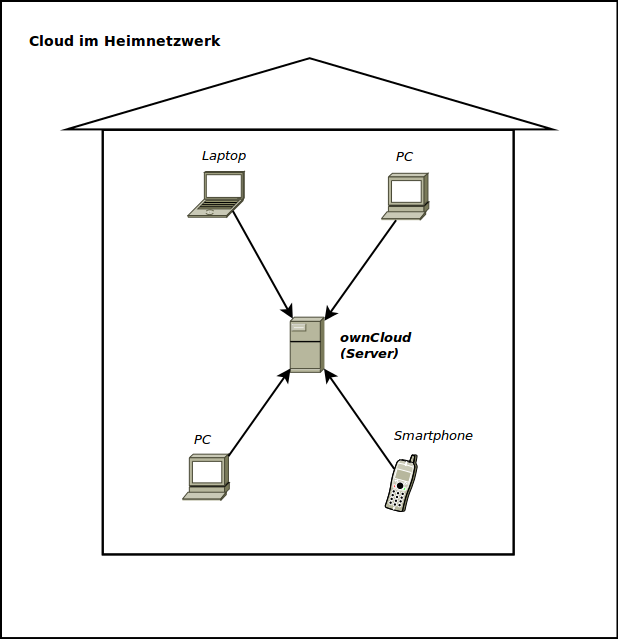
\includegraphics[scale=0.5]{images/owncloud_homenetwork}
\caption{ownCloud im Heimnetzwerk}
\end{figure}

\begin{figure}[h]
\centering
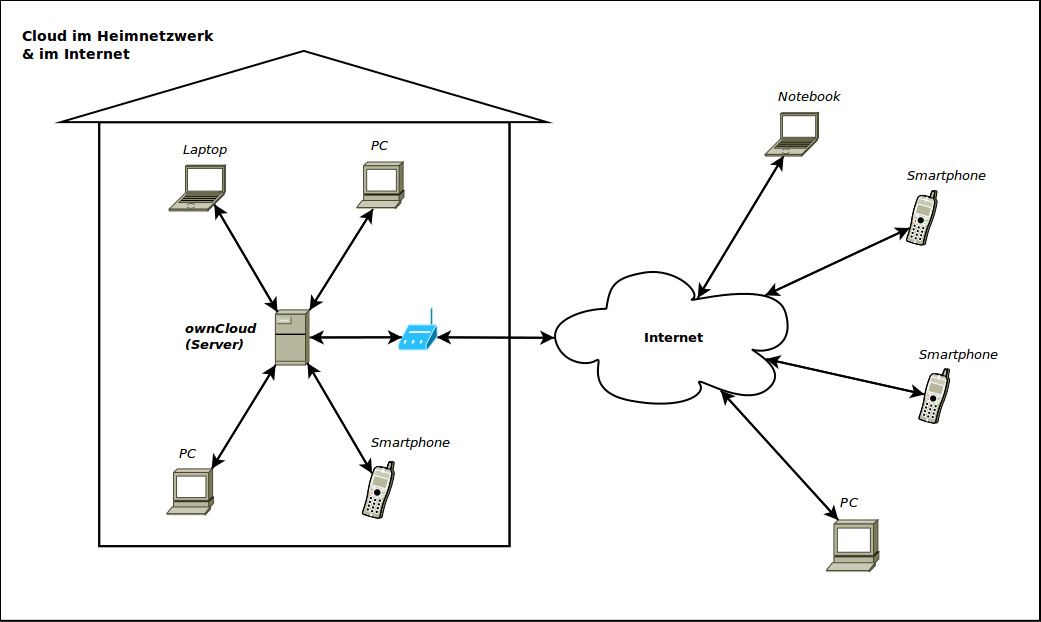
\includegraphics[scale=0.5]{images/owncloud_widenetwork}
\caption{ownCloud im Heimnetzwerk \& im Internet}
\end{figure}

\subsection{Vor- und Nachteile}
Grundsätzlich ist man bei ownCloud genau richtig, möchte man Herr seiner Daten sein. Was dadurch aber nicht vermieden werden kann ist eine gewisse Einarbeitungszeit bzw. ein gewisses technisches Know-How. Zusätzlich darf man auch nicht vergessen, dass die Cloud gewartet werden muss. Privatsphäre und Sicherheit haben ihren Preis und jede Privatperson bzw. jedes Unternehmen muss selbst entscheiden, wo die Prioritäten gesetzt werden. Die Cloud ist letztendlich nur so sicher, wie der Anwender sie gestaltet und selbst dann gibt es noch gewisse technologisch bedingte Einschränkungen.
Nachfolgend werden noch einmal einige Vor- und Nachteile stichwortartig aufgelistet, bevor das Experiment und dessen Ergebnisse beschrieben werden.
\\
\\
Vorteile
\begin{itemize}
\item Anwender ist der Souverän
\item Einsatz von Verschlüsselung bei Speicher und Übertragung
\item Kostenlos
\item Support durch Community
\item Open-Source-Software
\end{itemize}

Nachteile:
\begin{itemize}
\item Setzt gewisses technisches Know-How voraus
\item Wartung
\item u.U. Kauf eigener Hardware
\item Verbindungsgeschwindigkeit und Komfort u.U. nicht so hoch wie bei grossen Anbietern
\end{itemize}

\subsection{Experiment}
Dieses Kapitel schildert die Erfahrungen des Experiments, eine eigene Cloud mittels ownCloud einzurichten. Zum Schluss folgt ein Fazit und weitere Gedanken.

\subsubsection{Zielsetzung}
Das Ziel war es, eine Cloud für das heimische Netzwerk einzurichten. Das bedeutet, dass man von zu Hause aus auf die Cloud und die angebotenen Dienste zugreifen kann. Ausserhalb des heimischen Netzes ist dies dann nicht mehr möglich. ownCloud kann aber mit ein bisschen Mehraufwand so konfiguriert werden, dass auch dies möglich ist. Will man die eigene Cloud professionell nutzen, sollte dieser Mehraufwand definitiv betrieben werden. Als Computer kam dabei zu Testzwecken ein Raspberry Pi zum Einsatz. Das ist ein Einplatinen-Computer mit eher beschränkten Ressourcen, der nicht für grössere Projekte geeignet ist. Als Betriebssystem wurde eine für den Pi angepasste Version von Debian mit dem Namen Raspbian verwendet. Es handelt sich dabei um eine Linux-Distribution, die jedermann frei herunterladen und benutzen kann.

\subsubsection{Installation}
Die Installation selbst ging erstaunlich einfach vonstatten. Es gibt in den weiten des Internets viele Anleitungen und Tipps, die einem die Arbeit deutlich erleichtern. Mit ein bisschen Fleiss und Geduld hat man das nötige Know-How so sehr schnell zusammen. Zuerst mussten die Hardware- und die Softwarekomponenten ausgewählt werden. In beiden Bereichen hat man einen gewissen Spielraum. Dann ging es auch schon los mit dem Aufsetzen des Betriebssystems. Einmal korrekt eingerichtet, konnten die Software-Komponenten installiert werden, die neben der Cloud-Software für eine korrekte Ausführung benötigt werden. ownCloud selbst benötigte dann den kleinsten Aufwand. Innerhalb kürzester Zeit ist das Programm installiert und eingerichtet.
\\
\\
Standardmässig kann man sich mittels Webbrowser mit der Cloud verbinden. Die Bedienung geht dabei kinderleicht vonstatten. Es können mit wenigen Klicks alle Einstellungen vorgenommen und zusätzlich Funktionalitäten installiert werden. Alternativ lässt sich auf dem Computer, von dem man sich mit der Cloud verbinden will, eine Client-Programm installieren, mit dem der Einsatz der Cloud noch bequemer wird. Selbst für Smartphones gibt es eine App, die man installieren kann.

\subsubsection{Fazit}
Eine eigene Cloud zu erstellen mit ownCloud ging einfacher als erwartet. Hat man das benötigte Know-How einmal gesammelt, sollte der Einrichtungs-Prozess auch für einen Laien kein grosses Problem sein. Möchte man noch keine produktive Umgebung einrichten, sondern ownCloud zu Testzwecken ausprobieren, reicht ein alter Computer vollkommen aus. Auch die Anschaffung eines Raspberry Pis ist an dieser Stelle empfohlen. Zusammen mit dem nötigen Zubehör liegt der Preis immer noch unter 100 Franken. Die benötigten Linux-Kenntnisse sind möglicherweise eine gewisse Hürde, die den einen oder anderen abschreckt. Alternativen sind deshalb mit Windows und OS X vorhanden. Geduldige und Lernfreudige sollten aber auf Linux setzen, denn obwohl die Lernkurve zu beginn steil scheinen mag, kann man im Nachhinein Gebrauch von den vielen Vorteilen machen: Flexibilität, Performanz, Community, Sicherheit, keine Kosten u.v.m.
\\
ownCloud hat trotz der kurzen Testzeit einen sehr guten Eindruck hinterlassen. Die Bedienung ist leicht und ganz ähnlich, wie man es sich von anderen Programmen gewohnt ist. Das Programm bietet dabei eine Vielzahl von Zusatzdiensten, die man bei Bedarf nachinstallieren kann. Damit übersteigt der potenzielle Funktionsumfang von ownCloud sogar den der Grossen im Geschäft. Auch die Client-Programme für Computer, Smartphone und Tables liessen Freude aufkommen. 
\\
Möchte man Herr seiner Daten sein, ist ownCloud definitiv einen Versucht wert. Das im Rahmen des Experiments entstandene Handbuch führt den Anwender von der Anschaffung der Hardware bis zum finalen Einrichten der Cloud Schritt für Schritt durch den Prozess. Dass man dabei noch viel lernt, ist ein positiver Nebeneffekt.
Man findet das Handbuch im Anhang oder einzeln unter: ... xyz

% FIXME: Seite angeben

\subsection{Ausblick}
Reflexion über die Cloud und deren Zukunft - Zusammenhang zum Thema der Arbeit
